\documentclass[border=8pt]{standalone}
\usepackage{amsmath}
\usepackage{fontspec}
\setmainfont{Source Serif 4}
\usepackage{pgfplots}
\pgfplotsset{compat=1.18}
\definecolor{qbase}{RGB}{31,86,160}

\begin{document}
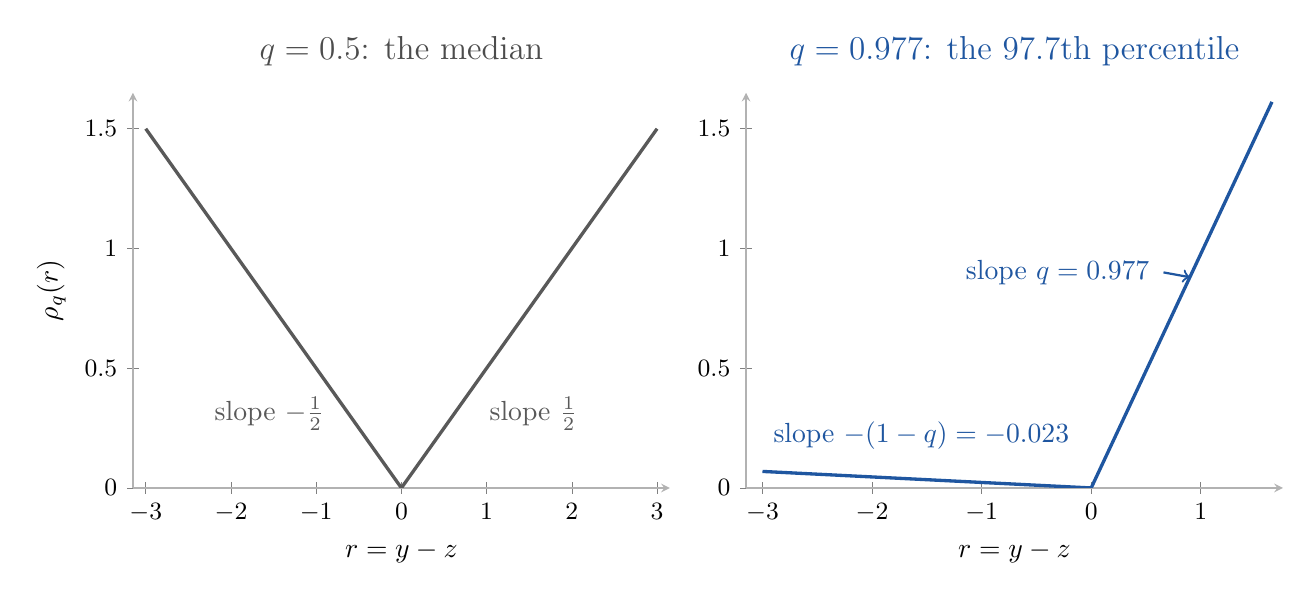
\begin{tikzpicture}
\begin{axis}[
  name=left,
  width=8.4cm, height=6.6cm,
  axis lines=left,
  title={$q = 0.5$: the median},
  title style={font=\large, black!70},
  xlabel={$r = y - z$}, ylabel={$\rho_q(r)$},
  xmin=-3.15, xmax=3.15, ymin=0, ymax=1.65,
  label style={font=\normalsize},
  tick label style={font=\small},
  axis line style={gray!60},
]
\addplot[domain=-3:0, samples=2, very thick, black!65] {0.5*(-x)};
\addplot[domain=0:3, samples=2, very thick, black!65] {0.5*x};
\node[black!65, font=\normalsize, anchor=north] at (axis cs:-1.55,0.42) {slope $-\tfrac{1}{2}$};
\node[black!65, font=\normalsize, anchor=north] at (axis cs:1.55,0.42) {slope $\tfrac{1}{2}$};
\end{axis}
\begin{axis}[
  at={(left.outer east)}, anchor=outer west, xshift=2mm,
  width=8.4cm, height=6.6cm,
  axis lines=left,
  title={$q = 0.977$: the 97.7th percentile},
  title style={font=\large, qbase},
  xlabel={$r = y - z$},
  xmin=-3.15, xmax=1.75, ymin=0, ymax=1.65,
  label style={font=\normalsize},
  tick label style={font=\small},
  axis line style={gray!60},
]
\addplot[domain=-3:0, samples=2, very thick, qbase] {0.023*(-x)};
\addplot[domain=0:1.65, samples=2, very thick, qbase] {0.977*x};
\node[qbase, font=\normalsize, anchor=south] at (axis cs:-1.55,0.12) {slope $-(1-q) = -0.023$};
\node[qbase, font=\normalsize, anchor=east] at (axis cs:0.62,0.9) {slope $q = 0.977$};
\draw[->, qbase, thick] (axis cs:0.66,0.9) -- (axis cs:0.9,0.88);
\end{axis}
\end{tikzpicture}
\end{document}
